%\title{LaTeX Portrait Poster Template}
%%%%%%%%%%%%%%%%%%%%%%%%%%%%%%%%%%%%%%%%%
% a0poster Portrait Poster
% LaTeX Template
% Version 1.0 (22/06/13)
%
% The a0poster class was created by:
% Gerlinde Kettl and Matthias Weiser (tex@kettl.de)
%
% This template has been downloaded from:
% http://www.LaTeXTemplates.com
%
% License:
% CC BY-NC-SA 3.0 (http://creativecommons.org/licenses/by-nc-sa/3.0/)
%
%%%%%%%%%%%%%%%%%%%%%%%%%%%%%%%%%%%%%%%%%

%----------------------------------------------------------------------------------------
%	PACKAGES AND OTHER DOCUMENT CONFIGURATIONS
%----------------------------------------------------------------------------------------

\documentclass[a0,portrait,posterdraft]{a0poster}
\usepackage[top=1in, bottom=1.25in, left=1.25in, right=1.25in]{geometry}

\usepackage{multicol} % This is so we can have multiple columns of text side-by-side
\columnsep=100pt % This is the amount of white space between the columns in the poster
\columnseprule=1.5pt % This is the thickness of the black line between the columns in the poster

\usepackage[svgnames]{xcolor} % Specify colors by their 'svgnames', for a full list of all colors available see here: http://www.latextemplates.com/svgnames-colors

\usepackage{graphicx} % Required for including images
\usepackage{tikz}
\usetikzlibrary{shapes,snakes,calc}
\usepackage[framemethod=tikz]{mdframed}
\usepackage{booktabs} % Top and bottom rules for table
\usepackage[font=normalfont,labelfont=bf]{caption} % Required for specifying captions to tables and figures
\usepackage{amsfonts, amsmath, amsthm, amssymb} % For math fonts, symbols and environments
\usepackage{wrapfig} % Allows wrapping text around tables and figures
\usepackage{enumitem}
\usepackage{soul}
\usepackage{xcolor}

\newcommand{\ctext}[3][RGB]{%
  \begingroup
  \definecolor{hlcolor}{#1}{#2}\sethlcolor{hlcolor}%
  \hl{#3}%
  \endgroup
}

\definecolor{mycolor}{rgb}{0.122, 0.435, 0.698}

\newmdenv[innerlinewidth=4.5pt, roundcorner=10pt,linecolor=mycolor,innerleftmargin=36pt,
innerrightmargin=36pt,innertopmargin=10pt,innerbottommargin=20pt]{mybox}

\newmdenv[innerlinewidth=4.5pt, roundcorner=10pt,linecolor=mycolor,innerleftmargin=16pt,
innerrightmargin=16pt,innertopmargin=16pt,innerbottommargin=16pt,backgroundcolor=black!7]{mybox2}

\setlist{nosep}
\renewcommand{\familydefault}{\sfdefault}
\begin{document}

%----------------------------------------------------------------------------------------
%	POSTER HEADER
%----------------------------------------------------------------------------------------

% The header is divided into two boxes:
% The first is 75% wide and houses the title, subtitle, names, university/organization and contact information
% The second is 25% wide and houses a logo for your university/organization or a photo of you
% The widths of these boxes can be easily edited to accommodate your content as you see fit

\begin{minipage}[b]{0.667\linewidth}
\VeryHuge \textbf{Monitoring and\\Visualizing BGP data} \\[.6cm]
\huge \textbf{{A. Kurth, Y. Lewash, S. Sontberg}}\\[2.4cm] % Author(s)
\Huge Project of Computer Systems and Telematics 2017\\[0.5cm] % Subtitle
\huge M. Nawrocki, M. W\"ahlisch\\[0.5cm] % Subtitle
\huge Freie Universit\"at Berlin, Institute of Computer Science, Germany\\[0.4cm] % University/organization
%\Large \texttt{\{marcin.nawrocki,m.waehlisch\}@fu-berlin.de} \\
\tiny \\
\end{minipage}
%
\begin{minipage}[b]{0.333\linewidth}

{
\includegraphics[height=4.9cm,interpolate]{LN_Logo.eps}}
\hspace{1cm}
{
\includegraphics[height=4.9cm,interpolate]{FULogo-RGB.pdf}}\\[2cm]
%{
\includegraphics[height=4.0cm,interpolate]{LN_Logo.eps}}
%{\includegraphics[height=4cm,interpolate]{Lehrpreis.jpg}}\
    \vspace{1.5cm}
\end{minipage}
%\vspace{1cm}

%\hline
%\vspace{1cm} % A bit of extra whitespace between the header and poster content
%\input{gan_graph}
%\hline
\vspace{.5cm} % A bit of extra whitespace between the header and poster content
%----------------------------------------------------------------------------------------
\begin{mybox}
\begin{multicols}{3} % This is how many columns your poster will be broken into, a portrait poster is generally split into 2 columns
\Large

\section*{Introduction}

The Internet is a web of thousands of interconnected networks, called Autonomous
Systems (AS). ASes are collections of routers with a coherent routing policy
controlled by a single administrative entity or domain (such as an Internet
service provider (ISP), a university, or a large company) and represent
connected groups of blocks of IP addresses, called IP prefixes. These IP address
aggregations determine the common path to each contained IP address within
these different networks.

\begin{center}\vspace{1cm}
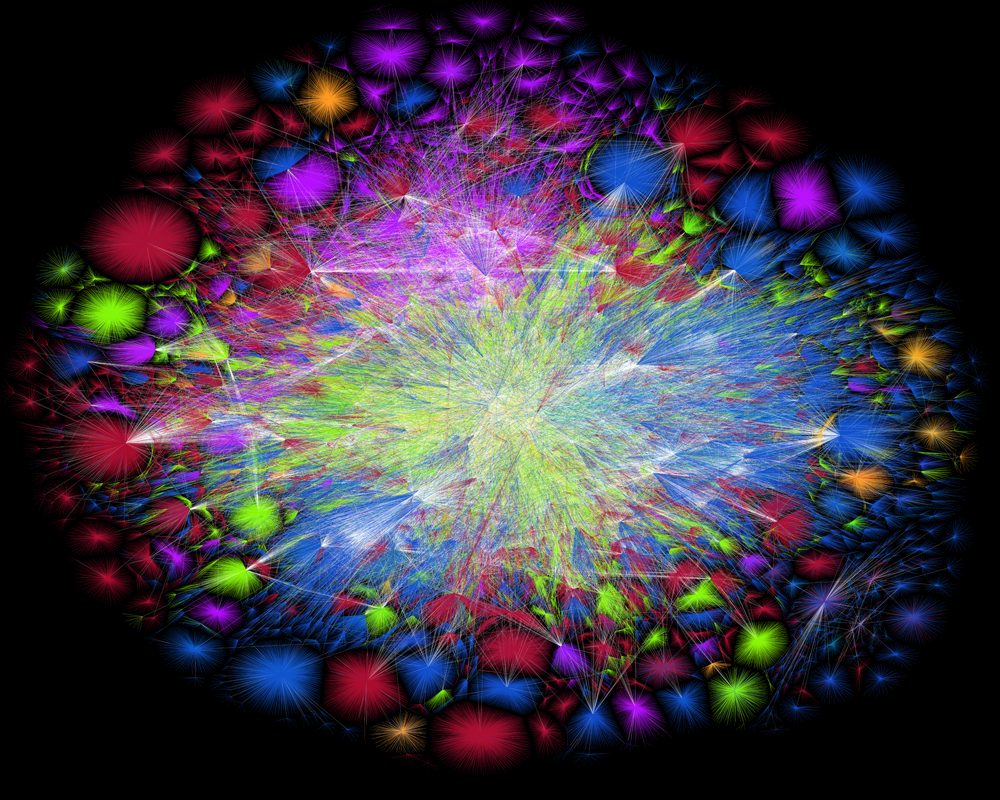
\includegraphics[width=0.9\linewidth,interpolate]{20150711_coords}
\captionof{figure}{
Visualization from the \emph{Opte Project} of the various routes on the Internet
captured in 2015.
Color Chart:\\
\color{white}\ctext[HTML]{1056CA}{North America (ARIN)}\color{black},
\ctext[HTML]{88F509}{Europe (RIPE)},
\color{white}\ctext[HTML]{A50FEB}{Latin America (LACNIC)}\color{black},
\color{white}\ctext[HTML]{A91034}{Asia Pacific (APNIC)}\color{black},
\color{white}\ctext[HTML]{E99330}{Africa (AFRINIC)}\color{black}.\\
Licenced under CC BY-NC 4.0.
}
\end{center}\vspace{1cm}

\noindent ASes use the Border Gateway Protocol (BGP) to establish connections
between each other. With BGP update messages an AS can announce changes in the
local database, advertise its IP prefix to neighboring ASes, and notify them of
new ``best'' (e.g. shortest) routes to other ASes on the Internet. These updates
are also used to withdraw old paths.

\section*{Prefix Hijacking and Outages}
However, any AS can also claim to own someone else's IP prefix and thereby
create invalid routes, as happened in 2008 when Pakistan Telecom announced a
prefix belonging to YouTube so that YouTube's traffic was hijacked on a global
scale.

\vfill
\columnbreak

\begin{center}\vspace{1cm}
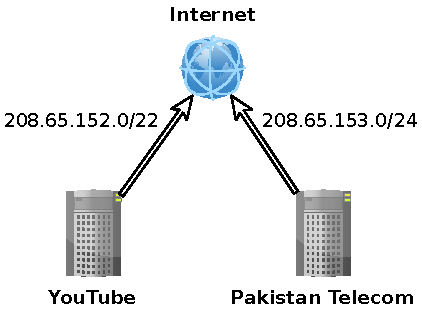
\includegraphics[width=0.9\linewidth,interpolate]{youtube_hijack.pdf}
\captionof{figure}{
Pakistan Telecom announced a more specific route than the one that was announced
previously by YouTube. Now most of the traffic would be redirected to the wrong
AS.
}
\end{center}\vspace{1cm}

\noindent While the damage in this case was only the loss of YouTube's
reachability and therefore quite easy to detect, other types of hijacking might
be even more serious than short outages. It is conceivable that the attacker
successfully masquerades as the real prefix owner or forwards the hijacked
traffic to the true destination while capturing all the transmitted data.

\section*{Securing BGP}

Since BGP itself lacks protection against such attacks (or just
configuration mistakes), the Internet Engineering Task Force (IETF) developed a
Resource Certification (RPKI) to validate the prefix origin and secure this
routing infrastructure. The holder of an address prefix can authorize ASes to
rightfully originate a prefix. This way the prefix of each BGP update can be
checked for origin validity before it is added to the route decision process.

\section*{BGP Data Collection}

There are different projects that gather BGP data from locations around the
world since 1997 and make it publicly available along with several tools to
monitor this data almost in real-time, analyze the historic development, or
academic research. Measuring BGP data is important to gain understanding about
structure and dynamics of the BGP ecosystem and the infrastructure of the
Internet.

\vfill
\columnbreak

\begin{center}\vspace{1cm}
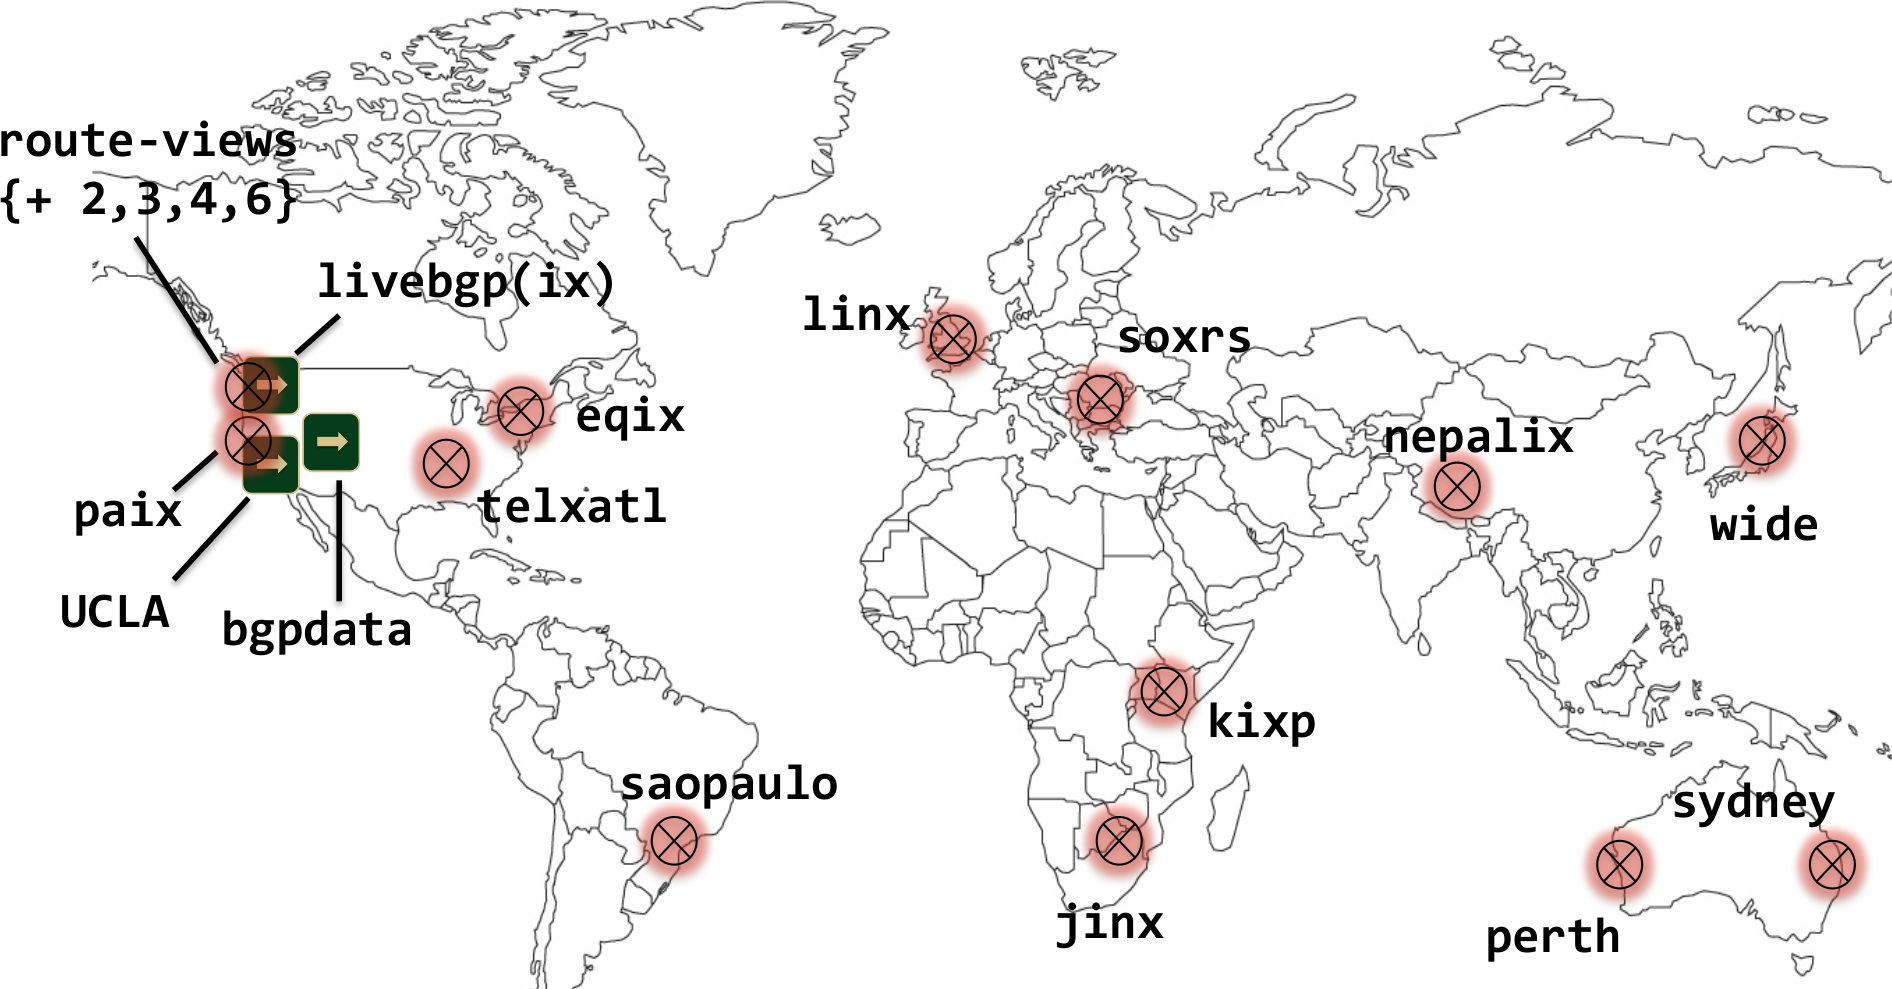
\includegraphics[width=0.9\linewidth,interpolate]{routeviews_33}
\captionof{figure}{
The \emph{RouteViews} project deploys 17 BGP route collectors worldwide and
archives the collected data continuously.
}
\end{center}\vspace{1cm}


\section*{Monitoring BGP Traffic}

With this data and tools available we can monitor and visualize BGP traffic with
regard to origin and path changes, new prefix announcements, or withdrawals to
allow a better understanding of routing decisions and disruptions.

\noindent In particular, using RPKI, it's possible to verify origins of IP
prefixes and compile statistics on prefix hijacking or incorrectly
configured attestations about authorized route announcements. Our tests have
shown that today at least up to 10 percent of monitored prefixes in this manner
can be validated with RPKI.

\vfill

\normalsize
\nocite{*}
\bibliographystyle{plain} % Plain referencing style
\bibliography{./bibliography.bib} % Use the example bibliography file sample.bib
% \section*{Bibliography} %% delete later if real bib exists
% \blinddescription

%----------------------------------------------------------------------------------------

\end{multicols}
\end{mybox}
\vfill
\begin{mybox2}
%\begin{center}
%\colorbox{black!20}{
%\begin{minipage}{.99\linewidth} 
\begin{minipage}{.17\linewidth} \small \centering
%\vskip.2em
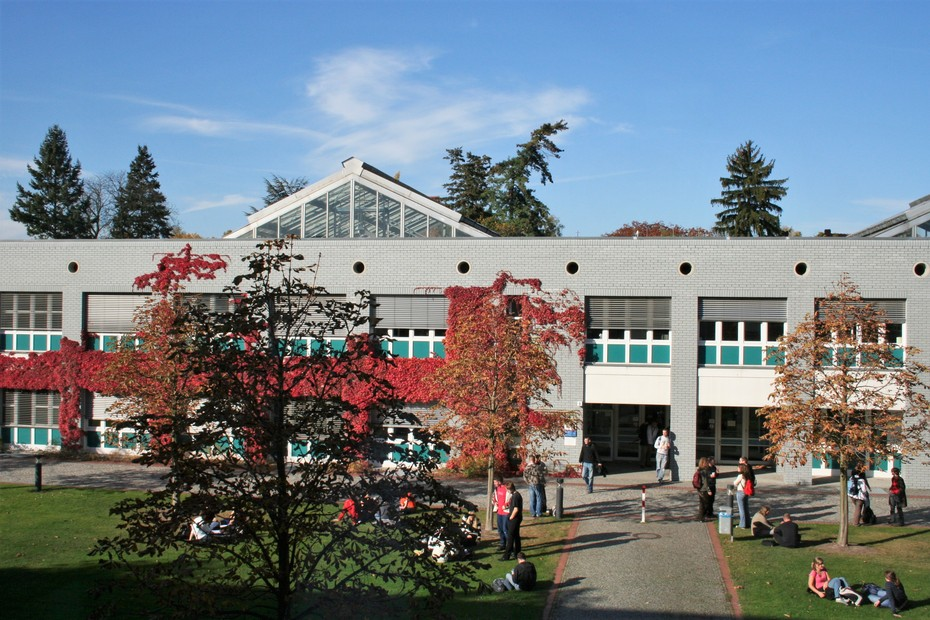
\includegraphics[width=.9\textwidth]{./inf_930} \\
{Institute of Computer Science}
\end{minipage}
\hfill
\begin{minipage}{.60\linewidth} \Large
Focus of research at CST (Computer Systems \& Telematics) group at Freie
Universit\"at Berlin (FU Berlin) is on mobile and wireless communications,
communication architectures and operating systems for embedded devices, and
quality of service aspects in communication systems.\par
%{\includegraphics[height=4cm,interpolate]{Lehrpreis.jpg}}\
\end{minipage}
\hfill
\begin{minipage}{.17\linewidth} \small \centering
%\vskip.2em
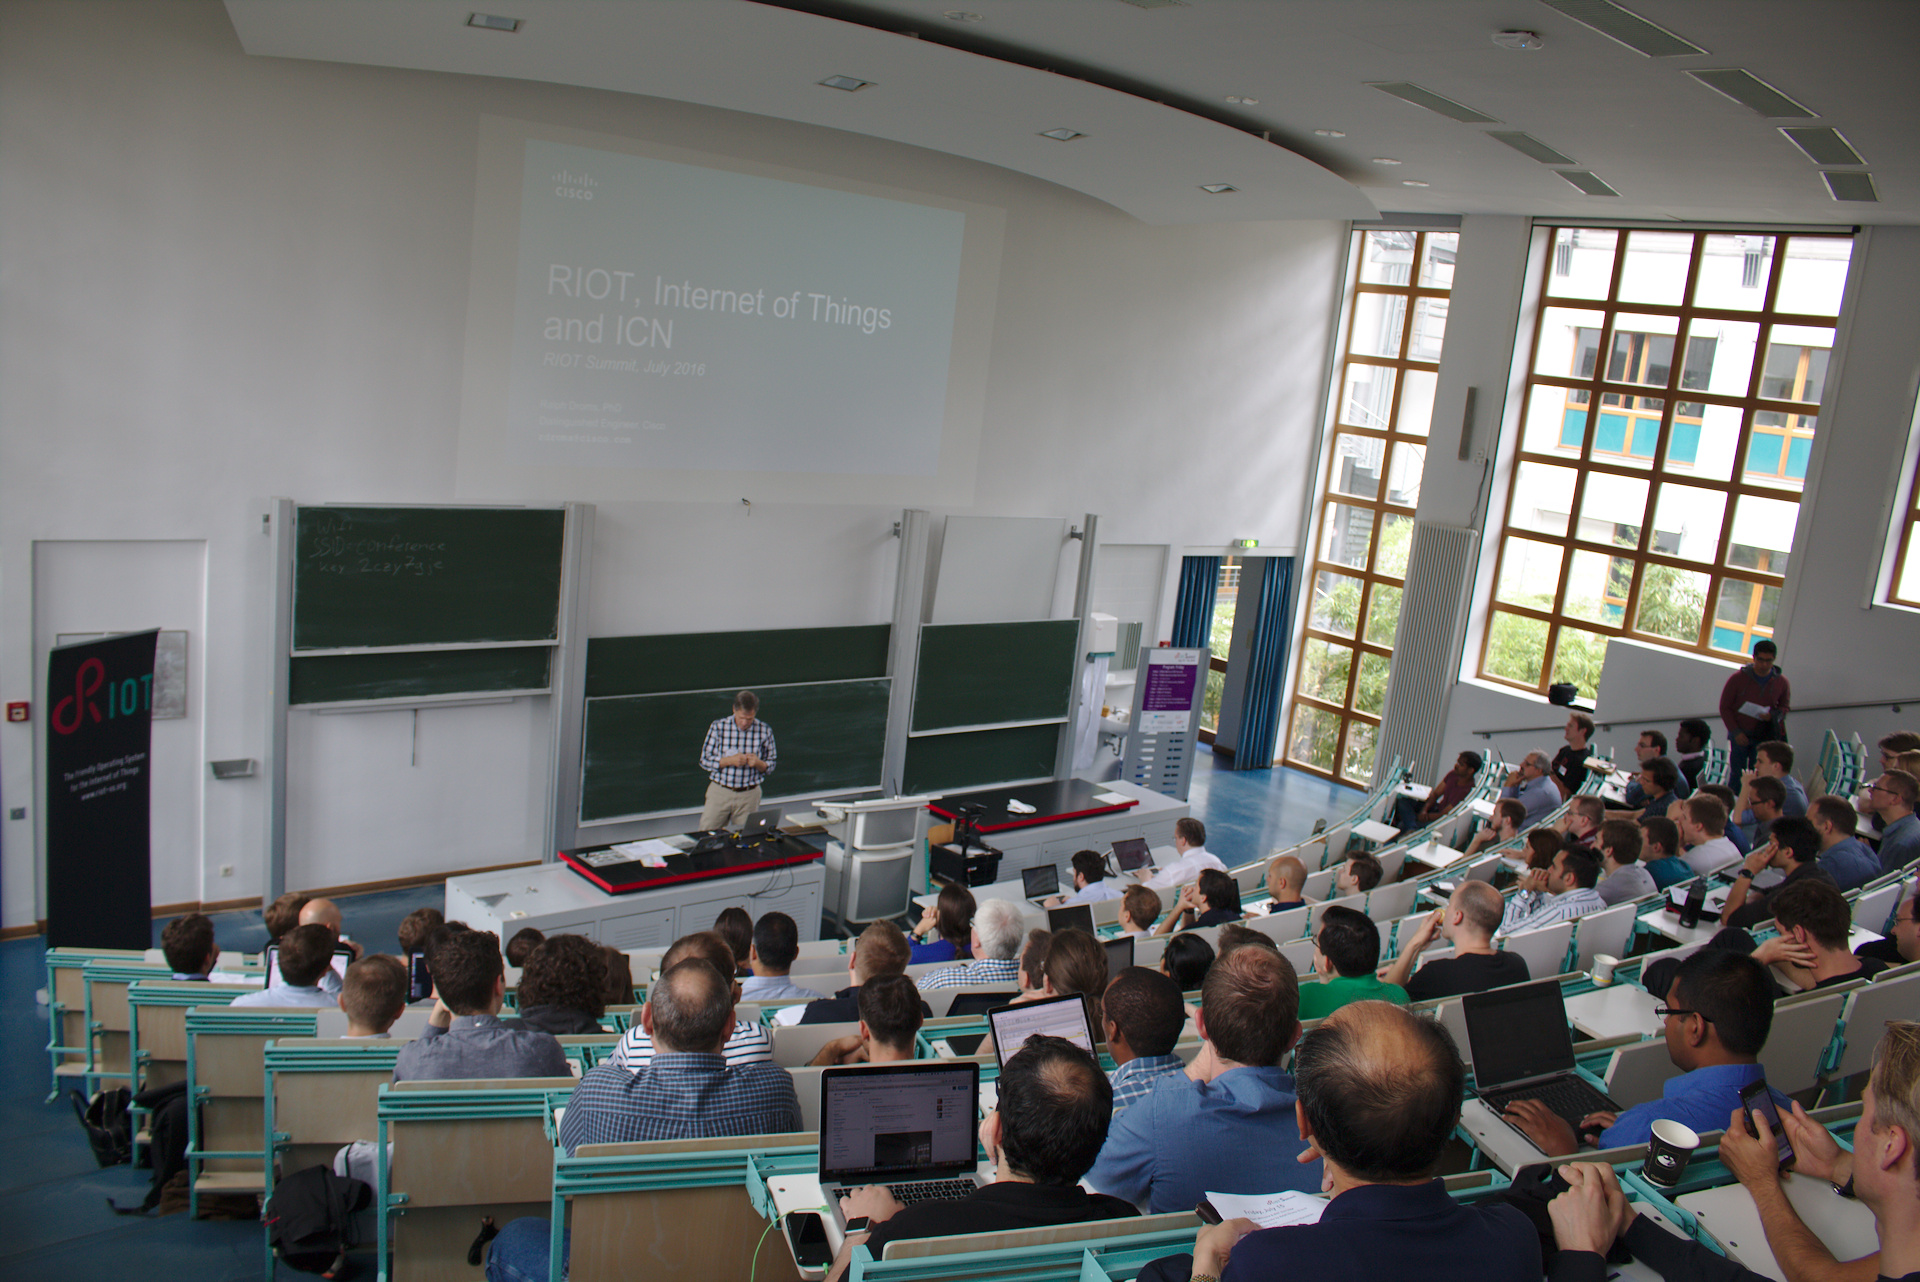
\includegraphics[width=.9\textwidth]{./IMG_0087} \\
{RIOT Summit 2016}
\end{minipage}
%\end{minipage}
%}
%\end{center}
\end{mybox2}
\end{document}
